\section{Meta-object Protocol and Separation of concerns}

\subsection{Open Implementation \& Meta-Object Protocol}

\subsubsection{Introduction}
"The work presented in this book is based ona \textbf{simple intuition}:

if \textbf{substrate systems} like programming languages, object
the details of the implementation of the base-level system are open
up to the meta-level system.
systems, databases or operating systems can \textbf{be tailored} to

meet particular application needs as they arise,

rather than having \textbf{to hack around} existing deficiencies,

application writers are better of."

Cit. Gregor Kiczales and Andreas Pæpcke

\subsubsection{System Awareness}
The computational reflection allows a system of observing and manipulating its components

\textbf{In particular}
\begin{itemize}
	\item the meta-level entities observe and manipulate the base-level entities, and
	\item these are NOT aware of being observed and manipulated.
\end{itemize}

\textbf{Therefore}:
\begin{itemize}
	\item there is a “black-box” use of the functionality of the base-level system
	\item the behavior of the base-level system and its structure can be dynamically modified, and
	\item the details of the implementation of the base-level system are open up to the meta-level system
\end{itemize}

\subsubsection{Black- and Gray-Box Approaches}

\begin{center}
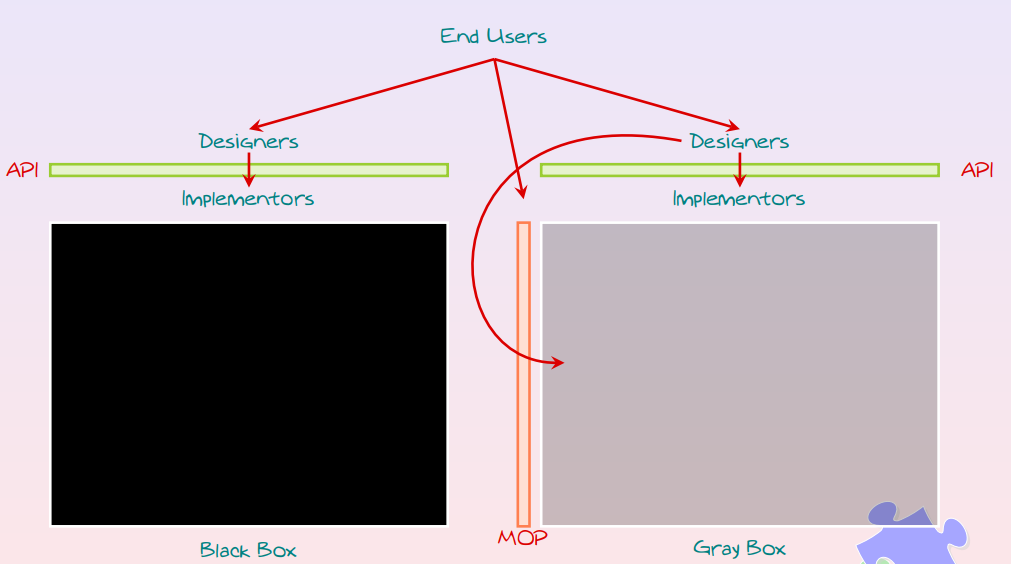
\includegraphics[scale=0.3]{6-black-and-gray-box-approaches}
\end{center}

\subsubsection{Black- and Gray-Box Approaches (Cont'd)}

\textbf{Black box}
\begin{itemize}
	\item the accesses to the system functionality is limited to the mechanisms provided by the adopted programming language
	\item an attempt of using the system functionality can raise an “application mismatch” when a component is used in the wrong way;
	\item flexibility is really limited
\end{itemize}

\textbf{Gray Box}
\begin{itemize}
	\item open implementation
	\item the component behavior can be adapted to our needs
	\item we can bypass the mechanisms provided by the programming language to access the system functionality
	\item we can re-class the objects respecting their use and behavior
\end{itemize}

\subsubsection{Kinds of Opening}

\textbf{(At least) 3 ways to open up the system details are possible}:

\begin{itemize}
	\item \textbf{introspection}, is the system ability of observing the state and the structure of the system itself
	\item \textbf{intercession}, is the system ability of modifying the behavior and the structure of the system itself;
	\item \textbf{invoke}, is the system ability of applying the system functionality
	
\end{itemize}

\subsubsection{Examples of MOP}

\textbf{Non-typed and interpreted programming languages}
\begin{itemize}
	\item Lisp
		- CLOS (Gregor Kiczales, 1991), ObjVLisp (Pierre Cointe, 1987), ABCL-R (Akinori Yonezawa, 1988)
\end{itemize}

\textbf{Typed and interpreted programming languages}
\begin{itemize}
	\item Java
		- java.lang.reflect (Sun, 1995)
		- OpenJava (Michiaki Tatsubori, 1999), Javassist (Shigeru Chiba, 2000), Reflex (Eric Tanter, 2001).
\end{itemize}


\textbf{Compiled programming languages}
\begin{itemize}
	\item C/C++
		- OpenC++ (Shigeru Chiba, 1993-1995), SOM/DSOM (Ira Forman, 1994), Iguana (Vinny Cahill, 1996).
\end{itemize}

\subsection{Separation of Concerns (SoC)}

\subsubsection{Introduction}

\begin{center}
\textbf{Complete Application}

=

\textbf{Core Functionality}

(e.g., banking applications: accounts, clients, operations, ...)

+

\textbf{Nonfunctional Concerns}

(security, persistence, distribution, exception handling, concurrency, ...)
\end{center}

Note that the separation between functional and nonfunctional is not so clear and neat.

\subsubsection{Introduction (Cont'd)}

\textbf{Traditionally}

\begin{itemize}
	\item separation of concerns is at design stage only
	\item source code is a mix of all concerns (functional and nonfunctional)
		- error prone
		- bad reusability and extensibility
\end{itemize}

\textbf{SoC aims at enabling such a separation in the implementation}

\begin{itemize}
	\item reflection, aspect-oriented programming
\end{itemize}

\subsubsection{Separation of Concerns Get as Reflective Activity}

\textbf{Reflection allows the designer of separating the functional aspects from the nonfunctional ones}

\textbf{Therefore, we get [*]}:
\begin{itemize}
	\item an augmentation of the functionality reuse
	\item an augmentation of the system stability; and
	\item the functional and nonfunctional aspects can be developed independently
\end{itemize}

[*] Walter Hürsch and Cristina Videira-Lopes. Separation of Concerns. TR. NU-CCS-95-03 Northeastern University. February 1995.

\subsubsection{Separation of Concerns Get as Reflective Activity (Cont'd)}

\begin{center}
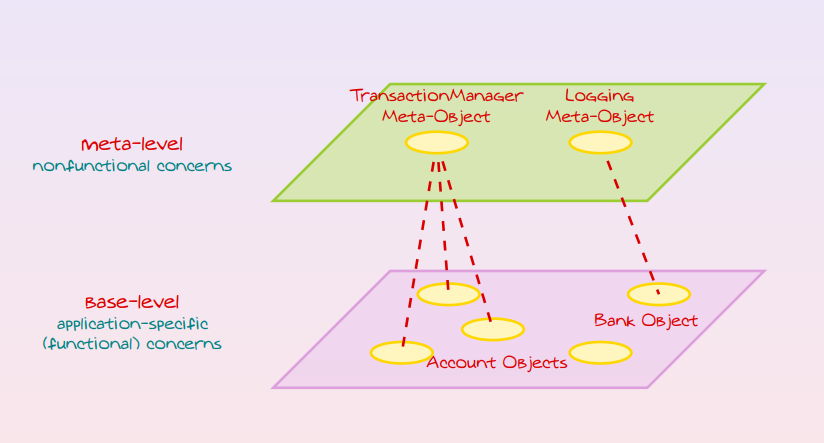
\includegraphics[scale=0.4]{7-separation-of-concerns-get-as-reflective-activity-contd}
\end{center}















